\documentclass{article} % For LaTeX2e
\usepackage{nips15submit_e,times}
\usepackage{hyperref}
\usepackage{url}
\usepackage{graphicx}
\graphicspath{ {images/} }
%\documentstyle[nips14submit_09,times,art10]{article} % For LaTeX 2.09


\title{Recommending Functions in Spreadsheets from the Fuse Corpus}


\author{
Shaown Sarker, Matthew Neal, Nisarg Vinchhi\\
Department of Computer Science\\
North Carolina State University\\
Raleigh, NC 27606 \\
\texttt{\{ssarker,meneal,nvinchh\}@ncsu.edu}
}

% The \author macro works with any number of authors. There are two commands
% used to separate the names and addresses of multiple authors: \And and \AND.
%
% Using \And between authors leaves it to \LaTeX{} to determine where to break
% the lines. Using \AND forces a linebreak at that point. So, if \LaTeX{}
% puts 3 of 4 authors names on the first line, and the last on the second
% line, try using \AND instead of \And before the third author name.

\newcommand{\fix}{\marginpar{FIX}}
\newcommand{\new}{\marginpar{NEW}}

\nipsfinalcopy % Uncomment for camera-ready version

\begin{document}


\maketitle

\begin{abstract}
Spreadsheets are the most widely used form of end-user programming. Although spreadsheets have a large array of functions built-in, the majority of spreadsheet users often do not utilize them in performing their tasks. To address this lack of function usage, we investigate recommender system technologies and consider two distinct approaches to a function recommender system for spreadsheets. In our work, we apply two variations of the collaborative filtering algorithm to produce personalized function recommendations for spreadsheet users by applying these algorithms on the Fuse spreadsheet corpus. We compare the performance of the algorithms used with a baseline of the Most Popular algorithm, also known as Linton's algorithm. In this paper, we present the feature extraction process from the spreadsheet corpus, the algorithms used and their comparative performance. Our cross validation results show that with a limited number of recommendations, our item-based recommendation algorithm performs significantly well compared to the baseline and the user-based approach.
\end{abstract}

\section{Introduction}
% The spreadsheet users are important.
Ko et al. define end-user programmers as people who are not professional software developers, but make use of the tools and processes that let them perform tasks similar to programming~\cite{ko2011state}. According to a study from 2005~\cite{scaffidi2005estimating}, nearly 23 million Americans use spreadsheets, constituting 30\% of the entire workforce. Spreadsheets are used not only for home and small businesses, but they are also very commonly used in industry. Almost 90\% of all analysts use spreadsheets to perform their calculations~\cite{winston2001executive}. Based on their numbers, spreadsheet users form the largest demographic within end-user programmers.

% There are lots of function, but people don't really use them.
Spreadsheet software comes with lots of functions built-in. Consider Microsoft Excel, the most widely used spreadsheet application, which has more than 300 functions\footnote{https://support.office.com/en-us/article/Excel-functions-by-category-5f91f4e9-7b42-46d2-9bd1-63f26a86c0eb}. But there are many situations where the user neglects using them. Let us consider the case of a spreadsheet user, Titus. Titus is a fourth grade teacher in an elementary school. At the end of the school year, he wants to calculate the class grades in Excel from all the test scores entered into his spreadsheet. Instead of using the arithmetic functions in Excel, he reaches for his hand-held calculator, and uses it to calculate and enter the grade for each student. This type of usage, not taking advantage of the functions in spreadsheets, is very common with users that lack awareness of the functionality~\cite{grossman2009survey} of the end-user programming tool being used.

% Address the issue with recommender systems.
Functionality awareness is important to accomplish new tasks as well as achieving efficient completion of existing tasks. Systems to recommend commands have been used successfully to improve functionality awareness in large and complex software applications~\cite{matejka2009communitycommands,murphy2012improving}. Recommender systems are used generally to produce a list of predictions based on the preference of an user and the similarity of preferences of other users. In recent years, recommender systems have become quite popular and have been applied successfully in multiple sectors of business~\cite{linden2003amazon} and academia~\cite{hsu2008personalized,mcnee2006don}. 

% Our contribution.
Our contribution in this paper -- we recommended functions in spreadsheets by applying two distinct variations of the collaborative filtering algorithm and compare the effectiveness of the recommendations using a cross validation based automated evaluation. We also compared their performance for recommending functions against another algorithm previously used for recommending commands in large software systems, the Most Popular algorithm~\cite{linton2000owl}. And we conclude by discussing how the results of our work can be used to create an Microsoft Excel plugin that can assist users to increase functional awareness by recommending functions they can use.

%% \subsection{Double-blind reviewing}

%% This year we are doing double-blind reviewing: the reviewers will not know 
%% who the authors of the paper are. For submission, the NIPS style file will 
%% automatically anonymize the author list at the beginning of the paper.

%% Please write your paper in such a way to preserve anonymity. Refer to
%% previous work by the author(s) in the third person, rather than first
%% person. Do not provide Web links to supporting material at an identifiable
%% web site.

%%\subsection{Electronic submission}
%%
%% \textbf{THE SUBMISSION DEADLINE IS June 5, 2015. SUBMISSIONS MUST BE LOGGED BY
%% 23:00, June 5, 2015, UNIVERSAL TIME}

%% You must enter your submission in the electronic submission form available at
%% the NIPS website listed above. You will be asked to enter paper title, name of
%% all authors, keyword(s), and data about the contact
%% author (name, full address, telephone, fax, and email). You will need to
%% upload an electronic (postscript or pdf) version of your paper.

%% You can upload more than one version of your paper, until the
%% submission deadline. We strongly recommended uploading your paper in
%% advance of the deadline, so you can avoid last-minute server congestion.
%%
%% Note that your submission is only valid if you get an e-mail
%% confirmation from the server. If you do not get such an e-mail, please
%% try uploading again. 

%% \subsection{Keywords for paper submission}
%% Your NIPS paper can be submitted with any of the following keywords (more than one keyword is possible for each paper):

%% \begin{verbatim}
%% Bioinformatics
%% Biological Vision
%% Brain Imaging and Brain Computer Interfacing
%% Clustering
%% Cognitive Science
%% Control and Reinforcement Learning
%% Dimensionality Reduction and Manifolds
%% Feature Selection
%% Gaussian Processes
%% Graphical Models
%% Hardware Technologies
%% Kernels
%% Learning Theory
%% Machine Vision
%% Margins and Boosting
%% Neural Networks
%% Neuroscience
%% Other Algorithms and Architectures
%% Other Applications
%% Semi-supervised Learning
%% Speech and Signal Processing
%% Text and Language Applications

%% \end{verbatim}

\section{Related Work}
Researchers have been studying and analyzing spreadsheets to better comprehend the activity of users and design better tools to assist them. Previous research has focused on extracting structured domain information from spreadsheets~\cite{hermans2010automatically} and visualizing spreadsheets using dataflow diagrams~\cite{hermans2011breviz} to enhance understandability of spreadsheets. For improving the maintainability and quality of spreadsheet formulas, systems have been implemented to detect code smells in formulas and refactor them to resolve the detected smells~\cite{hermans2014detecting}. In contrast, our work attempts to increase the functionality awareness in spreadsheets by suggesting functions.

Moreover, some research has used recommender systems to help users of a large software system with vast set of functionality to learn these functionalities. One of the early notable attempts is the OWL system~\cite{linton2000owl} developed by Linton et al., which suggests commands to Microsoft Word users based on the Most Popular algorithm. In OWL, commands are recommended to an individual if she is not using certain commands at all, but the community is using them on a frequent basis. The underlying assumption of this system is that all users of a software system have a similar command usage distribution.

Matejka and his colleagues developed a collaborative filtering-based approach called CommunityCommands~\cite{matejka2009communitycommands} to recommend commands in AutoCAD, a computer aided drafting software. Similarly based on usage history, Murphy-Hill and colleagues studied several existing recommendation algorithms to recommend commands in Eclipse. The approach that we propose in this paper, focuses on the algorithm used by OWL as a baseline and the user-based and item-based variations of the collaborative filtering algorithm used by CommunityCommands.

Both of the algorithms used in our work require a source of function usage preferences for the spreadsheet users' community. Although there are existent spreadsheet corpora like Enron~\cite{hermans2014enron} and EUSES~\cite{fisher2005euses} which have been valuable sources for spreadsheet analysts and researchers alike, in this paper we look into a very recently extracted spreadsheet corpus: Fuse~\cite{barik2015fuse}. Unlike Enron and EUSES which are very domain specific, Fuse contains a more diverse and much larger body of spreadsheets. Fuse is also reproducible, thus the recommender system in our work can leverage of a larger spreadsheet corpus if needed, which can be extracted by the system developed by Fuse's creators.

The rest of the paper is organized as follows: we describe the feature extraction process by which we retrieved the user preferences to be used for the recommender systems, along with a brief explanation of how collaborative filtering and the baseline algorithms work. We then describe our evaluation strategy followed by the results observed. In the end, we discuss any threat to validity of our work and the future work that can be extended based on our contribution.

\section{Methodology}
\subsection{Feature Extraction}
The Fuse spreadsheet corpus consists of nearly two hundred fifty thousand distinct spreadsheets. The creators of Fuse extracted the meta information for these spreadsheets in JSON format using Apache POI library which includes the user that created and last modified the spreadsheet, and the frequency of the functions being used in the spreadsheet. We identified almost seven thousand individual users by combining the created by and last modified by meta information along with the domain name where the spreadsheet was originally extracted. This gave us a collection of nearly seven thousand user vectors, such that the vector $V$ for an individual user consists of cells, where each cell $V_{i}$ represents the usage frequency of the function $f_{i}$. Consider the sample user identifying key, user vector tuple below:
\begin{center}
   \texttt{('Greenfield, Laura\#Greenfield, Laura\#www.cde.state.co.us', \{'SUM': 8, 'Plus': 179, 'Divide': 179\})}
\end{center}
Here, this user has used 'SUM', 'PLUS', and 'DIVIDE' functions 8, 179, and 179 times respectively over her spreadsheets in Fuse.

\subsection{Collaborative Filtering}
Collaborative filtering is a method of making automatic predictions (filtering) about the interests of a user by collecting preferences or taste information from many users (collaborating). The core concept of collaborative filtering is to apply a nearest neighbor method between a user's preferences and the preference of a large user community, and provide the user with recommendations by extrapolating based on how her selection or preference relates to that of the community. In our work, we look at the user-based and item-based variations of collaborative filtering.

\subsubsection{User-based Collaborative Filtering}
Although collaborative filtering can be applied in many ways, the approaches falling under the category of user-based collaborative filtering are composed of mainly two distinct steps~\cite{breese1998empirical} - find the users with similar preference patterns to that of the input user, and then use the preference of the similar users to obtain predictions for the input user.

We use the user vectors extracted in the feature extraction step here. To compensate for the overriding influence of functions that are frequently used by a large number of users, we use a weighting function named 'function frequency inverse user frequency' (ff-iuf) which is similar to the well-known 'term frequency inverse document frequency' (tf-idf) technique used to determine the importance of a word or term to a document in a collection~\cite{sparck1972statistical}. The ff-iuf for an user $i$ and a function $j$ can be defined as:
\begin{center}
   $ff\mbox{-}iuf_{ij} = \alpha \cdot ff_{ij} \cdot iuf_{ij}$
\end{center}

Where, $\alpha$ is a tuning parameter, and
\begin{center}
   \begin{displaymath}
   ff_{ij} = \frac{\mbox{Frequency of function j for user i}}{\mbox{Total frequency of all functions used by user i}}
   \end{displaymath}
\end{center}

\begin{center}
   \begin{displaymath}
   iuf_{ij} = \log \frac{\mbox{Total number of users}}{\mbox{Number of users that use function j}}
   \end{displaymath}
\end{center}

In the weighted vectors, a higher value signifies that function is used frequently by that individual user, but that function is used by a relatively small portion of the total users.

To obtain the users with similar function usage to the input user, we used cosine similarity function that measures the angle between the users' vectors. When the cosine similarity is near zero, the angle between the vectors are closer to a right angle and the vectors are not very similar. On the other hand, if this value is close to 1, then the vectors are nearly colinear and are quite similar. By comparing the cosine similarity value between the input user and the other vectors, we determine the $n$ most similar users, where $n$ is another tuning paramter in our system.

After we have the similar users, we recommend the top $m$ functions that are used by the similars but not by the input user, where $m$ is another tuning parameter. The recommended functions are ordered by their cumulative function frequency as described above over the $n$ similar users.

\subsubsection{Item-based Collaborative Filtering}
In this approach, using the ff-iuf weighted vectors used above, we define a vector for each function $j$, where a cell $i$ in the vector is the ff-iuf value for user $i$ and function $j$.

Then we generate a function-to-function two dimensional similarity matrix $M$, where the matrix element $m_{jk}$ represents the cosine similarity value between function vectors for function $j$ and $k$.

Given the input user, we recommend $m$ functions that are not used by the user, ordered by their similarity score from the similarity matrix, where for all function $i$ and function $k$, such that $i$ is not used but $k$ is used by input user:
\begin{center}
   \begin{displaymath}
   \mbox{similarity score for function i}, s_i = average(m_{ik})
   \end{displaymath}
\end{center}


\subsubsection{Most Popular}
Linton and colleagues introduced the Most Popular algorithm in their OWL~\cite{linton2000owl} system which recommended commands in Microsoft Word. The Most Popular algorithm suggests functions that are most widely used by the community but not used by the input user. To implement this algorithm, we took the cumulative frequency count for each function over all the spreadsheets in Fuse, which is referred to as the \textit{confidence level} of a function. When we are given an input user vector as described in the previous section, this algorithm recommends functions with highest confidence level values, excluding any function that is present in the user's input vector.

The underlying assumption of this algorithm is that the functions most frequently used by the community are also the most useful functions. For this reason, this algorithm has an advantage over collaborative filtering - it can recommend functions to users whose function usage history is not known (the input vector consists of entirely zeros). However, this algorithm suffers from lack of personalization, as it does not take into consideration the usage frequencies of the functions in the input user vector.

\section{Evaluation}
For evaluating the system based on the algorithms in the previous section, we used the k-folds cross validation technique, which enabled us to evaluate our system using the existing feature vectors extracted from the Fuse corpus. We used a 14 fold cross validation, splitting the entire set of ~7,000 user vectors in 14 slices and treating a single slice as testing set and the rest as our training set.

In our cross validation, we took a single user vector from the testing set as input vector. In this input vector, we removed a function at random and retrieved the recommendations for this modified input vector. If the set of recommendations contained the removed function, then we counted this as a successful recommendation. The success rate was represented as a percentage of each individual testing set. The overall 14-fold cross validation success rate was calculated as a mean of these individual 14 success rates.

\section{Results}
For item-based approach, we had one tuning parameter - $m$, the number of functions recommended. We used four different values for $m$: 1, 3, 5, 10. The bar graph in figure \ref{fig:itemresults} shows the comparative overall success rate for the different values for the number of recommendations retrieved.

\begin{figure}[h]
\begin{center}
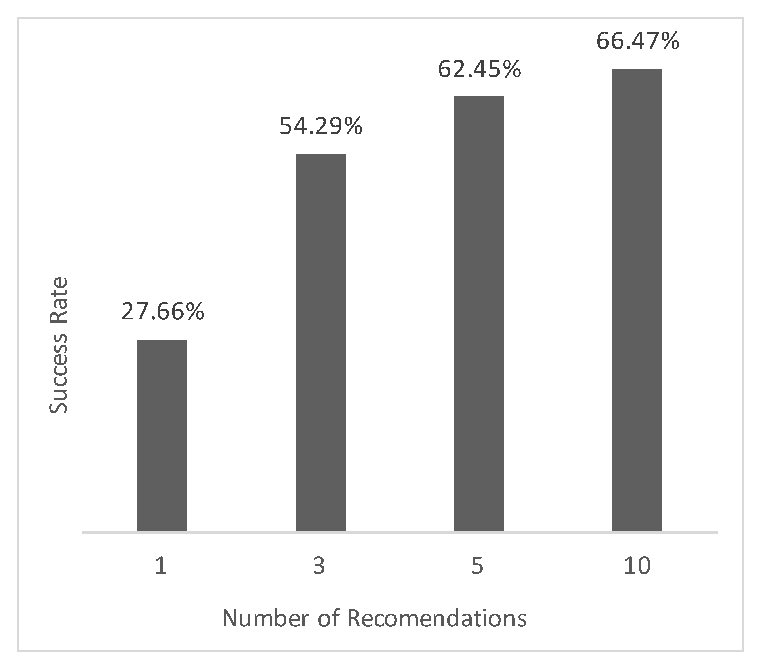
\includegraphics[height=6cm,width=8cm]{Item}
\end{center}
\caption{Item-based CF: number of recommendations vs success rate}
\label{fig:itemresults}
\end{figure}

\begin{center}
   \texttt{Under Construction}
   \begin{itemize}
      \item Specify tuning parameters - number of similar users and number of recommendations retrieved for user-based CF along with bar chart graphics to display results.
      \item Specify the tuning paramters - number of recommendations retrieved for baseline algorithm along with bar chart graphics to display results.
      \item Comparative results graphics featuring cluster bar graphics to show overall results for all three algorithms.
   \end{itemize}
\end{center}

\section{Discussion}
From the results of the item-based collaborative filtering algorithm, we can conclude that the recommendations become more effective as we increase the number of recommendations retrieved $m$, but the effectiveness of the recommendations start to pleateau after the value of $m$ reaches 5.
\begin{center}
   \texttt{Under Construction}
   \begin{itemize}
      \item Discuss results for user-based cf.
      \item Discuss comparative performance against baseline.
      \item Address any threats to validity.
   \end{itemize}
\end{center}

\section{Future Work}
One of the salient limitations of the recommendation systems used in this work was that the function usage rate and diversity was quite low in the Fuse spreadsheet corpus, where only a very small percentage of the spreadsheets contained function usage. This however can be alleviated considerably by incorporating other existing spreadsheet corpus like Enron~\cite{hermans2014enron} and EUSES~\cite{fisher2005euses} into the extracted user function vectors used in our algorithms.

Spreadsheet files, being static, do not contain any temporal or sequential information regarding function discovery. Given the function discovery sequence information, it will be possible to apply a number of other recommendation systems resulting in a much higher success rate. For example, the discovery variations of the algorithms as described by Murphy-Hill and colleagues, which produced the recommendations with the highest success rates in their automated evaluation~\cite{murphy2012improving}. In the discovery variations of the algorithms, instead of using function frequency based vectors, users' vectors consist of discovery patterns that reflect the order in which an user discovers functions in spreadsheets. The collaborative filtering version with discovery finds user vectors with similar discovery patterns and recommends functions the similar users have discovered but the user has not. In the most popular algorithm with discovery, the most discovered function in the community is recommended to an user who has not discovered that function yet.

Although we used an automated method to evaluate our system, it cannot replace the recommendations being evaluated by real life spreadsheet users. This type of evaluation can prove how much useful the recommendations actually are. It is possible to conduct a study, where we generate recommendations based on spreadsheet users in the industry and have the actual owners of the spreadsheets evaluate their personalized function recommendations. Alternatively, we can also measure the effectiveness of our recommendations by observing if the users accept the recommendations by using the function being recommended.

\bibliographystyle{unsrt}
\bibliography{report.bib}

\end{document}
